\section{Podsumowanie}
Niniejsza praca opisuje nowe podejście do automatycznego generowania twarzy
ludzkiej z wykorzystaniem gramatyk kształtu. Za zastosowaniem gramatyk kształtów
przemawia fakt, że pozwalają na uzyskanie zadowalających rezultatów oraz na
łatwą parametryzację kształtów przez nią generowanych. Wydaje się, że jest to
najlepsze podejście do problemu automatycznego generowania kształtów parametrycznych.
\subsection{Napotkane trudności}
Podczas realizacji pracy napotkaliśmy kilka trudności natury koncepcyjnej oraz
implementacyjnej. Pierwszym problemem był dobór
odpowiedniego sposobu reprezentacji geometrii. Początkowo mieliśmy tworzyć model
w taki sam sposób, jak jest tworzony przez grafików -- wychodzić z prostego
modelu prostopadłościanu i kolejnymi regułami modyfikować prostopadłościan do
uzyskania odpowiedniego modelu. Jest to najlepszy możliwy sposób, jeśli w
rezultacie chcemy otrzymać siatkę (ang. mesh). Stwarza jednak pewne problemy w
implementacji, szczególnie jeśli chodzi o organiczne elementy -- brak ostrych
krawędzi. Problem ten można rozwiązać poprzez wykorzystanie powierzchni
b-sklejanych~\footnote{http://www.cs.mtu.edu/~shene/COURSES/cs3621/NOTES/surface/bspline-construct.html}
(ang. b-spline surface). Metoda mogłaby dawać dobre rezultaty lecz
również jest ciężka w implementacji -- szczególnie operacje logiczne takie jak
suma, część wspólna powierzchni. Ostatecznie zdecydowaliśmy się na opis przy
pomocy prostych matematycznych obiektów oraz wykonywanych na nich przekształceń.
Taki opis pozwala na wyrenderowanie dobrej jakości obrazu oraz bezproblemowe
przenoszenie zapisu matematycznego do przestrzeni wokselowej.

Drugą napotkaną trudnością, wynikającą ze sposobu opisu modelu jaki
wybraliśmy, było w miarę wierne odwzorowanie ludzkiej głowy. Mając do
dyspozycji jedynie sfery, cylindry, sześciany itp. nie da się uzyskać idealnego
modelu. Brak edytora, który wyświetlając w oknie zdjęcia, pozwalałby również na
pobieranie określonych wymiarów, utrudniał poprawną parametryzację. Ostatecznie
oparto się o wymiary wyznaczone bez udziału programu.

\subsection{Dalszy rozwój}
Projekt wykonany w ramach praktycznej części pracy jest tylko zalążkiem tematu.
Do prezentacji wygenerowanego obiektu zastosowaliśmy przestrzeń wokselową,
głównie dzięki łatwości operacji na niej. Próbowaliśmy wizualizować obiekt za
pomocą ray-tracingu, co dało lepszą jakość generowanego obrazu. Zastosowanie
tego algorytmu uniemożliwiło jednak dodawanie filtrów wygładzających (np.
usuwanie ostrych krawędzi). Nie mniej jednak wydaje się nam, że ostatecznie
ray-tracing byłby lepszym rozwiązaniem i warto byłoby w przyszłości skupić się
na takim sposobie przenoszeniu obiektu do 2D.

Kolejną wartą poruszenia kwestią jest sposób generacji bryły na podstawie zdjęć.
Jedną z koncepcji, nad którą się zastanawialiśmy było dostosowywanie obiektu do
zdjęć na zasadzie dopasowywania geometrii do obrazu:
\begin{enumerate}
 \item dopasowanie koloru obiektu do koloru obrazu -- binaryzacja obrazu z
 przedziału koloru skóry, uśrednienie koloru zbinaryzowanego obszaru
 $\longrightarrow$ kolor obiektu 3D;
 \item za pomocą np. algorytmów genetycznych dopasowanie parametrów obiektu 3D
 tak, aby różnica pomiędzy fotografią a obrazem wygenerowanym z gramatyki
 kształtu była jak najmniejsza;
 \item wykonanie drugiego kroku dla coraz to bardziej szczegółowych parametrów
 gramatyki.
\end{enumerate}
Na ilustracji~\ref{klaudia01} zaprezentowany jest pierwszy z wymienionych
etapów:
\begin{figure}[h!]
  \centering
  \subfloat[Obraz źródłowy]{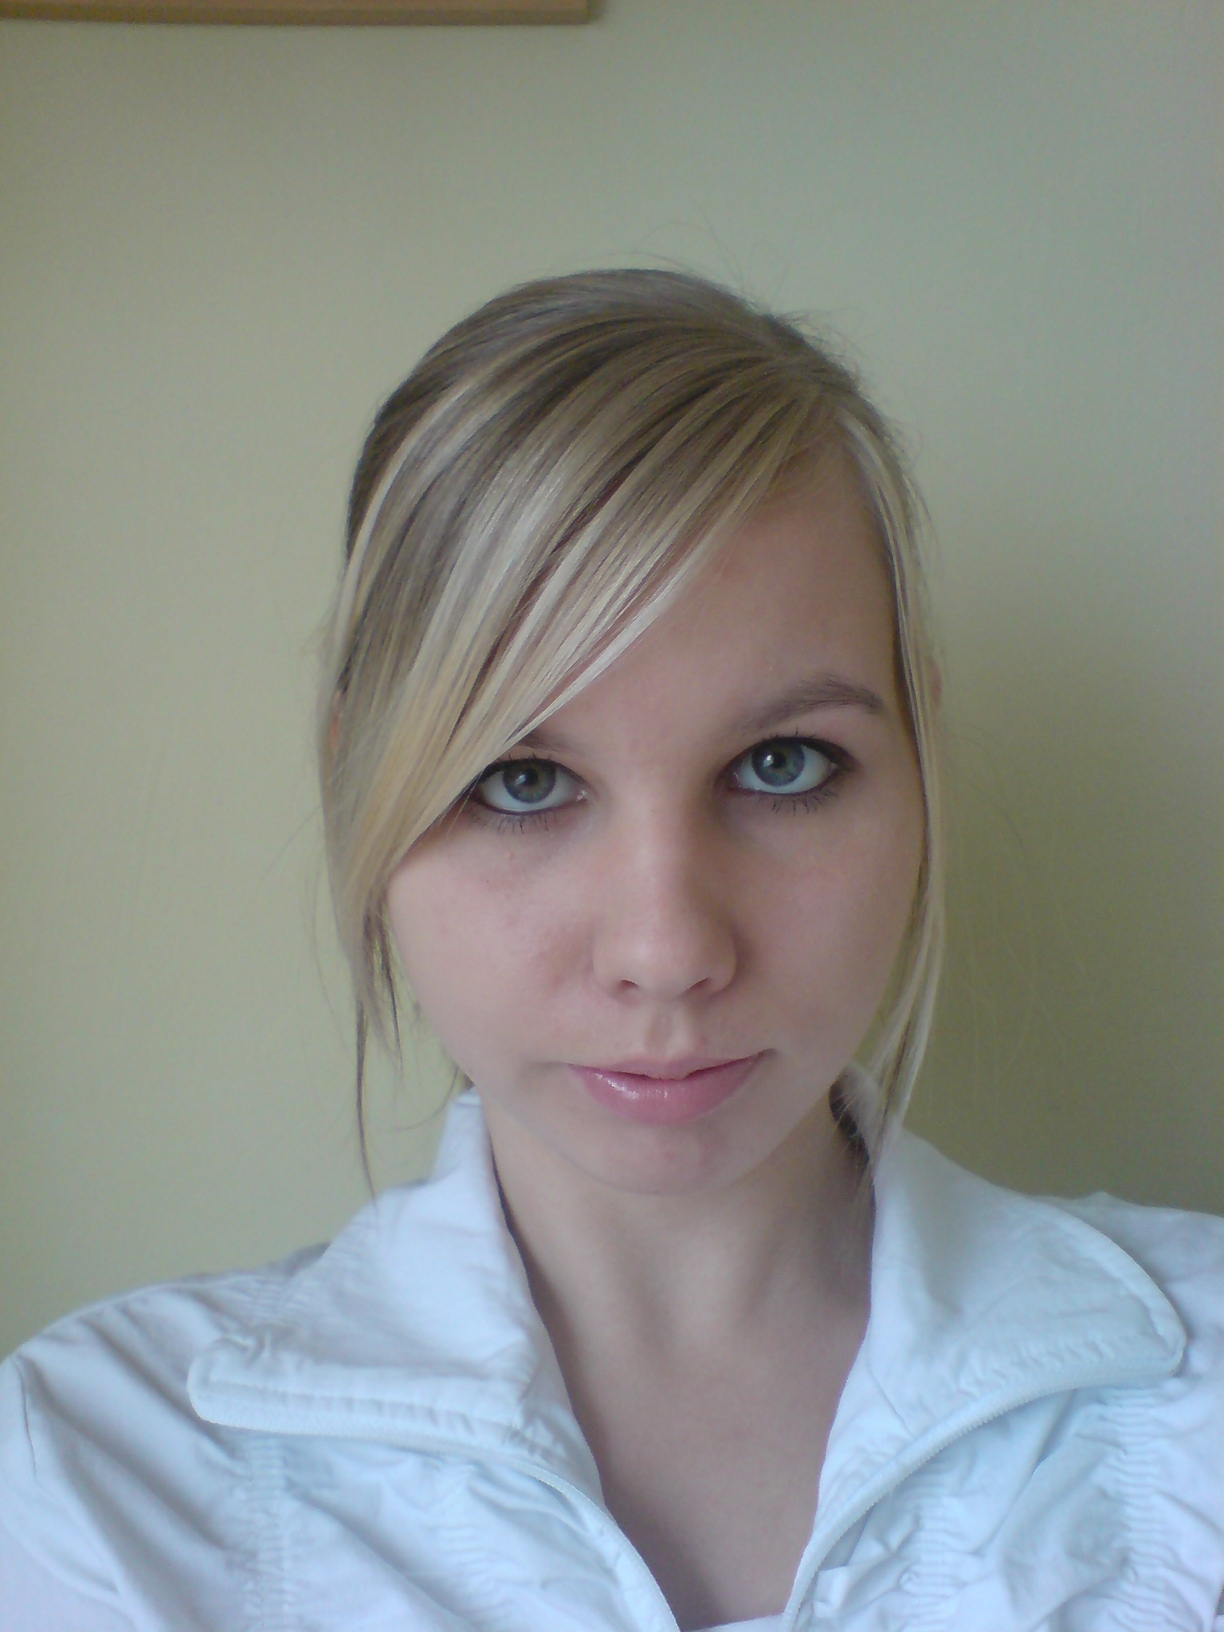
\includegraphics[width=6cm]{images/klaudia01.jpg}}
  \subfloat[Obszar zbinaryzowany]{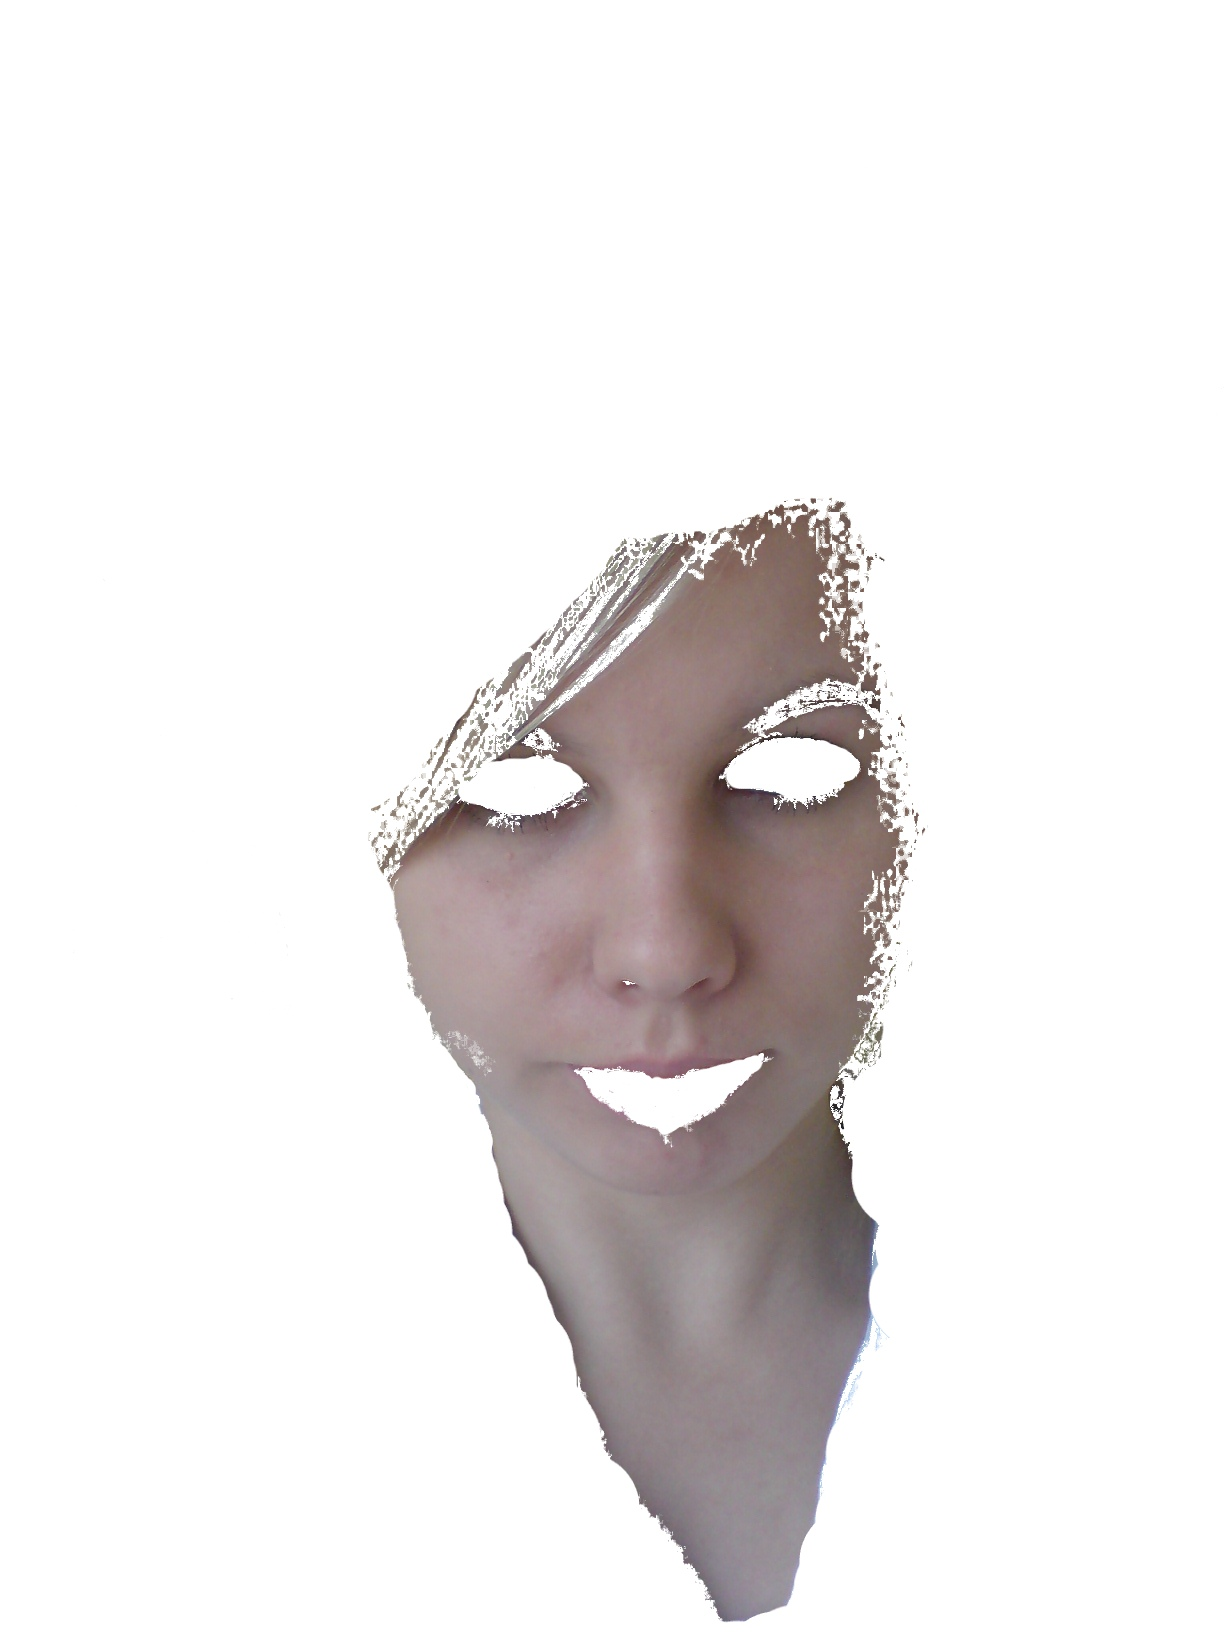
\includegraphics[width=6cm]{images/klaudia02.jpg}}
  \subfloat{\label{average}
\includegraphics[width=1cm]{images/klaudia03.png}}
  \caption{Kolejne etapy wyznaczania koloru obiektu, \ref{average}~uśredniony
  kolor zbinaryzowanego obszaru (źródło własne).}
  \label{klaudia01}
\end{figure}
Gdy mamy wyznaczony średni kolor obrazu - nakładamy ten kolor na obiekt 3D z
gramatyki i automatycznie sterujemy parametrami gramatyki (algorytmami
genetycznymi). Po każdym kroku porównujemy obraz wyrenderowany z obrazem
źródłowym.

Podczas przeprowadzania symulacji z użyciem różnych gramatyk unaocznił się
problem z wydajnością zastosowanych algorytmów. Najbardziej oczywistym
sposobem na poprawę wydajności jest dodanie obsługi wielowątkowości. Specyfika
programu pozwala na zastosowanie wielowątkowości w różnych częściach
aplikacji: renderingu (każdy wątek renderuje inny fragment obrazu),
przetwarzaniu drzewa gramatyki (kolejne podwęzły wykonywane w osobnym wątku).

Edytor do wyznaczania miar na podstawie wczytanych zdjęć mógłby w znaczący
sposób pomóc projektantowi gramatyki. Mając do dyspozycji proporcje głowy,
odległości pomiędzy wybranymi częściami można by dużo łatwiej tworzyć gramatykę
kształtu.

Ostatnią i chyba najistotniejszą zmianą w ramach tej pracy jest zmiana sposobu
generacji bryły. Pierwsze podejście jakie rozpatrywaliśmy, a mianowicie
modyfikacja siatki z prostego modelu (prostopadłościanu), byłaby najbardziej
efektowna, dawałaby najlepsze rezultaty i mogłaby generować np. bryłę low-poly.
\subsection{Wnioski}
Wygląd wygenerowanego obiektu nie przypomina do złudzenia ludzkiej głowy ale
otwiera drogę do nowego sposobu generowania organicznych modeli w świecie 3D. Po
przeprowadzeniu testów okazało się, że wybrany przez nas sposób reprezentacji
geometrycznej gramatyki posiada wiele ograniczeń oraz tworzy strukturę, którą
trudno jest rozbudowywać. Warto zainteresować się możliwością zaimplementowania
innego sposobu reprezentacji geometrii bądź technik hybrydowych oraz bardziej
rozbudowanych elementów modyfikujących geometrię.
Wykorzystanie podstawowych obiektów geometrycznych jak sfera, sześcian,
cylinder do budowania głowy okazało się niewystarczające jednak pozwoliło na
przetestowanie mechanizmu tworzenia prostej głowy w oparciu o gramatykę
kształtu.
